\chapter{Results}
\label{results}


\section{Implementation of the percolator algorithm}
- Reimplementierung funktioniert wie Original $\rightarrow$ Dafür müsste man irgendwie C Percolator zum testen nutzen können. \\
The implementation of feature normalization yielded an increase in the number of confident PSMs found, as the y-axis and legend of figure~\ref{fig:feature_normalization} show. This type of plot is explained in~\autoref{lab:results:pseudo_rocs}. The performance of Pycolator with feature normalization is better from the first iteration on, and increases until iterations~7~or~8, when the results converge. Without feature normalization, the area under the pseudo ROC increases until iteration~3, when it begins to oscillate. \\
\renewcommand{\baselinestretch}{0.9}
\begin{figure}
	\normalsize
	\centering
	\begin{subfigure}{0.49\textwidth}
		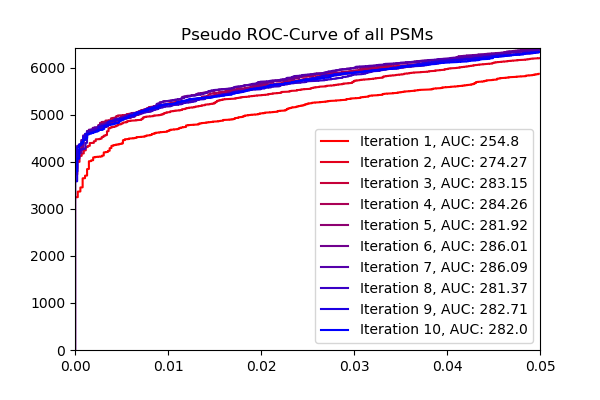
\includegraphics[width = \textwidth]{figures/noNorming.png}
		\caption{}
		\label{fig:before_feature_normalization}
	\end{subfigure}
	\hfill
	\begin{subfigure}{0.49\textwidth}
		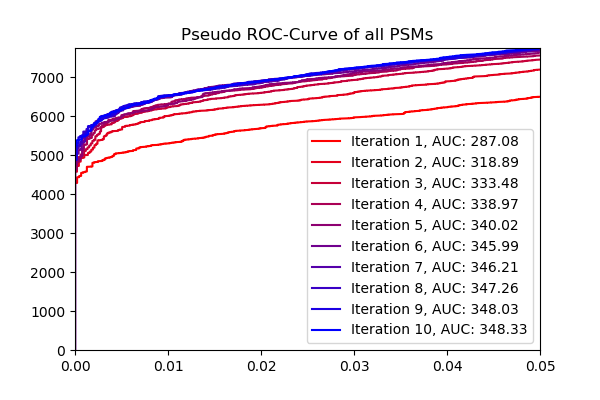
\includegraphics[width = \textwidth]{figures/norming.png}
		\caption{}
		\label{fig:after_feature_normalization}
	\end{subfigure}
	\caption[Results of implementing feature normalization]{Result of Pycolator before~(\ref{fig:before_feature_normalization}) and after~(\ref{fig:after_feature_normalization}) the implementation of feature normalization. }
	\label{fig:feature_normalization}
\end{figure}
\renewcommand{\baselinestretch}{1}

\section{Adapting Percolator to Cross-link Identification}
\label{lab:results:pseudo_rocs}
An example of the plots created by Pycolator are shown in figure~\ref{fig:results:pseudo_rocs}. One plot shows the pseudo ROC of the non-cross-linked PSMs in every iteration, one the cross-linked and one all of the PSMs. In each, every iterations pseudo ROC curve has its own color, ranging from red in iteration~1 to blue in iteration~10. The colors can be assigned from the legend, which also shows the area under the depicted pseudo ROC curve. Every curve ranges from q-values~$0$~to~$5\%$ and the y-axis is scaled appropriate for the data. As explained in~\ref{lab:background:roc}, a higher and more left (pseudo) ROC curve is better. Thus, as one can see in figure~\ref{fig:results:pseudo_rocs_all}, the result of Pycolator improves over almost every iteration.\\
\renewcommand{\baselinestretch}{0.9}
\begin{figure}
	\normalsize
	\centering
	\begin{subfigure}{0.49\textwidth}
		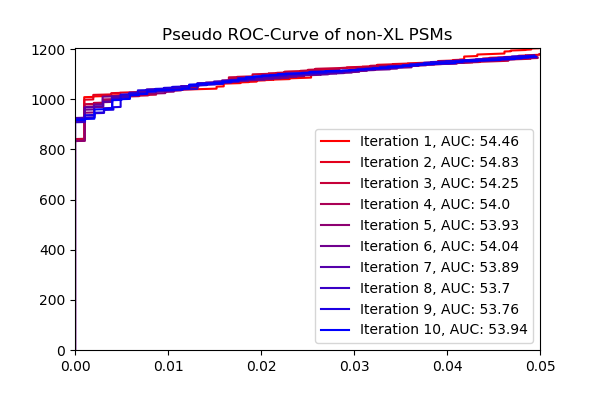
\includegraphics[width = \textwidth]{figures/pseudoROC_non-XL.png}
		\caption{}
		\label{fig:results:pseudo_rocs_nXL}
	\end{subfigure}
	\hfill
	\begin{subfigure}{0.49\textwidth}
		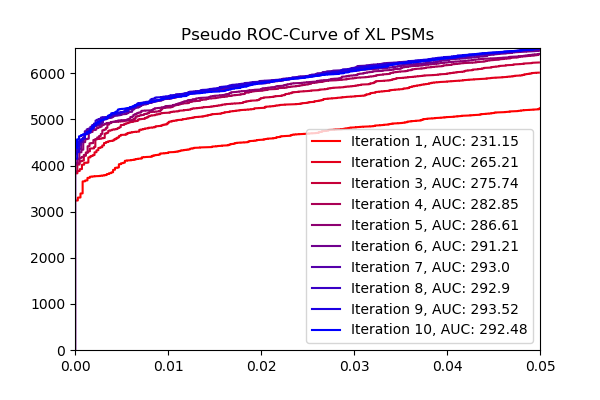
\includegraphics[width = \textwidth]{figures/pseudoROC_XL.png}
		\caption{}
		\label{fig:results:pseudo_rocs_XL}
	\end{subfigure}
	\hfill
	\begin{subfigure}{0.49\textwidth}
		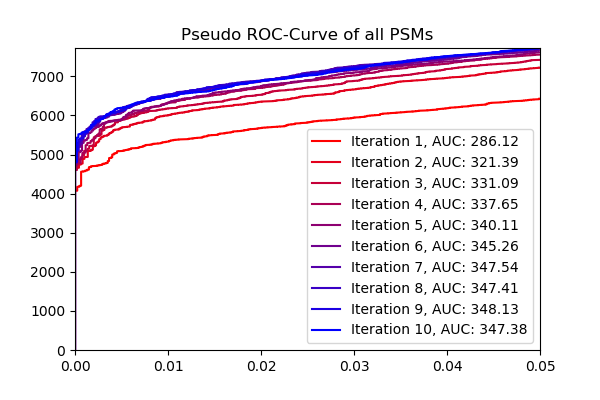
\includegraphics[width = \textwidth]{figures/pseudoROC_all.png}
		\caption{}
		\label{fig:results:pseudo_rocs_all}
	\end{subfigure}
	\caption[Examples for pseudo ROC curves as produced by Pycolator]{Example of the plots output by Pycolator, generated by running with default parameters on the given dataset~(\ref{lab:matmet:dataset}). \ref{fig:results:pseudo_rocs_nXL}~shows the result of non-cross-linked PSMs, \ref{fig:results:pseudo_rocs_XL}~that of cross-linked and~\ref{fig:results:pseudo_rocs_all} that of all PSMs in the dataset.}
	\label{fig:results:pseudo_rocs}
\end{figure}
\renewcommand{\baselinestretch}{1}

\subsection{Different Ranks}
\label{lab:results:ranks}
Figure~\ref{fig:before_optimalranking} shows the pseudo ROCs of Pycolator before the implementation of the new mechanism. \ref{fig:all_ranks} was plotted when Pycolator used all PSMs available, meaning all ranks, and only at the end lower ranking PSMs than 1 were excluded. \ref{fig:only_rank_one} is the result of running Pycolator only with rank 1 PSMs of the given dataset~\ref{lab:matmet:dataset} and~\ref{fig:optimalranking} shows the final result with the new feature.\\
As one can see, without the new mechanism Pycolator gradually improves the area under the curve and takes $5$ and $4$ iterations to roughly converge when given every PSM or only rank 1 PSMs to train respectively. This can be seen by the AUC results after every iteration or the ROC curves themselves. The end result, however, is better when removing the lower ranking PSMs right at the beginning (AUC of $345.79$) instead of in the end (AUC of $343.21$ after dropping the lower ranking PSMs). Since in the latter case Pycolator ended with an AUC of $343.79$ as one can see in~\ref{fig:all_ranks}, dropping the PSMs slightly worsened the end result. With the new feature, the algorithm takes about $5$ iterations to converge, then performs a jump and again improves over two iterations. The end result, an AUC of $348.13$, is higher than both alternatives. Multiple runs yielded very similar results. 
\renewcommand{\baselinestretch}{0.9}
\begin{figure}
	\normalsize
	\centering
	\begin{subfigure}{0.49\textwidth}
		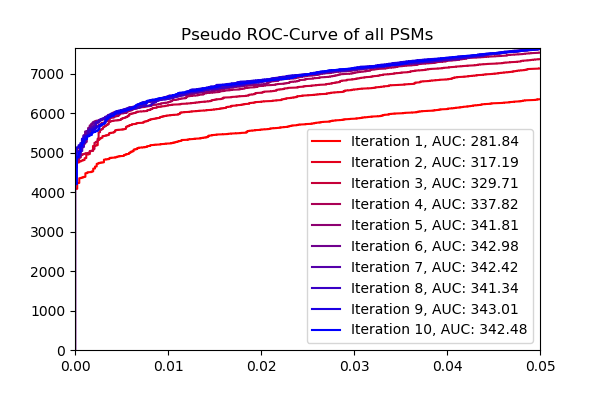
\includegraphics[width = \textwidth]{figures/allRanks.png}
		\caption[Result of dropping lower ranks at the end]{The resulting pseudo ROCs (explained in~\ref{lab:results:pseudo_rocs}) if Pycolator is given every PSM regardless of its rank. Lower ranking PSMs are only dropped in the end, which results in a final AUC of $343.21$.}
		\label{fig:all_ranks}
	\end{subfigure}
	\hfill
	\begin{subfigure}{0.49\textwidth}
		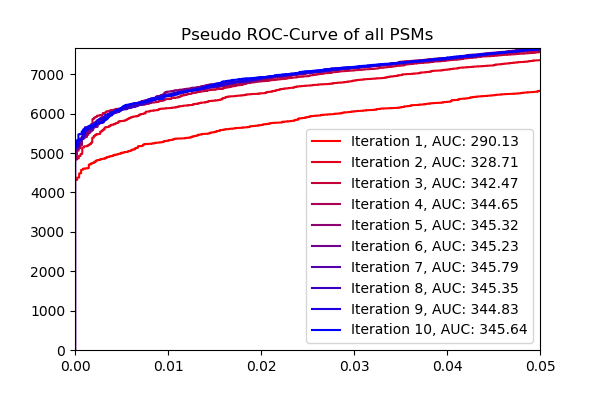
\includegraphics[width = \textwidth]{figures/onlyFirstRank.png}
		\caption[Result of dropping lower ranks at the start]{The resulting pseudo ROCs (explained in~\ref{lab:results:pseudo_rocs}) if Pycolator is given only the top scoring peptide for every spectrum. Lower ranking PSMs are dropped before running the algorithm.}
		\label{fig:only_rank_one}
	\end{subfigure}
	\begin{subfigure}{0.75\textwidth}
		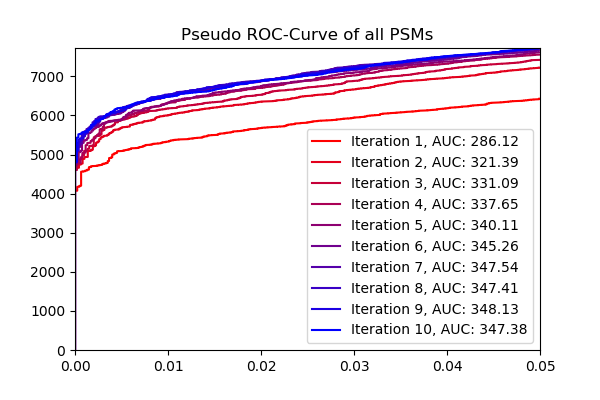
\includegraphics[width = \textwidth]{figures/optimalRanking.png}
		\caption[Result of the new ranking procedure]{The resulting pseudo ROCs (explained in~\ref{lab:results:pseudo_rocs}) if Pycolator is run with the newly implemented feature. It first trains with every PSM available, and after the results converge, lower ranking PSMs are dropped. Then, the algorithm runs for some more iterations.}
		\label{fig:optimalranking}
	\end{subfigure}
	\caption[Results of strategies regarding different ranks]{Results of running Pycolator with different strategies as to how lower ranking PSMs are dealt with.}
	\label{fig:before_optimalranking}
\end{figure}
\renewcommand{\baselinestretch}{1}

\subsection{Characteristics of Cross-linked PSMs}
\subsubsection{Proportions of Different Classes}
\label{lab:results:proportions}
- Verhältnis Targets:Decoys und XL:non-XL verringt die Streuung: MinMaxMedian Auswertungen\\
Maintaining the proportion of classes works as intended, as figure~\ref{fig:results:prop_code} shows. It depicts the proportion of targets~(t) to decoys~(d) in each of the three outer splits and the whole dataset.\\
\renewcommand{\baselinestretch}{0.9}
\begin{figure}
	\normalsize
	\centering
	\begin{subfigure}{\textwidth}
		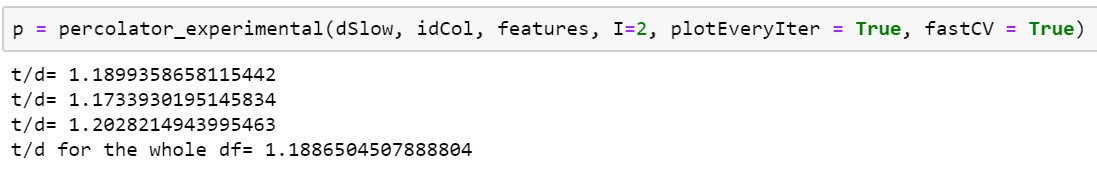
\includegraphics[width = \textwidth]{figures/prop_not_kept_code.jpg}
		\caption{Ratios of target to decoy PSMs in each of the three splits, ranging from $1.173$ to $1.203$, while the ratio is $1.8865$ in the whole dataset.}
		\label{fig:results:prop_not_maintained}
	\end{subfigure}
	\begin{subfigure}{\textwidth}
		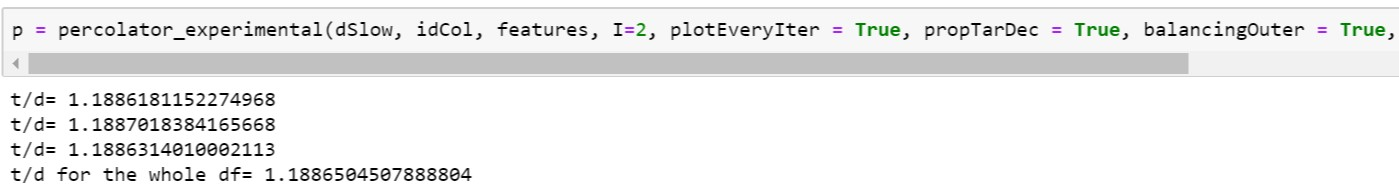
\includegraphics[width = \textwidth]{figures/prop_kept_code.jpg}
		\caption{Ratios of target to decoy PSMs in each of the three splits, ranging from $1.18862$ to $1.18870$, while the ratio is $1.18865$ in the whole dataset.}
		\label{fig:results:prop_maintained}
	\end{subfigure}
	\caption[Maintaining proportions works as intended]{The log of two test runs of Pycolator. It calculated and output the ratio of targets to decoys in every of the outer split and the whole dataset. In~\ref{fig:results:prop_maintained} the proportions were maintained, and in~\ref{fig:results:prop_not_maintained} they were not.}
	\label{fig:results:prop_code}
\end{figure}
\renewcommand{\baselinestretch}{1}
The evaluation produced the results shown in figure~\ref{fig:results:maxminmedian}. The corresponding areas under the curve are listed in table~\ref{tab:results:maxminmedian}.
\renewcommand{\baselinestretch}{0.9}
\begin{figure}
	\normalsize
	\centering
	\begin{subfigure}{0.49 \textwidth}
		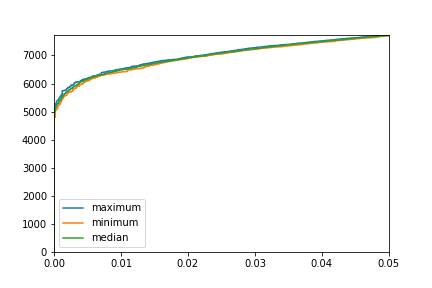
\includegraphics[width = \textwidth]{figures/MaxMinMedian_no_balancing.png}
		\caption{}
		\label{fig:results:maxminmedian_not_maintained}
	\end{subfigure}
	\hfill
	\begin{subfigure}{0.49 \textwidth}
		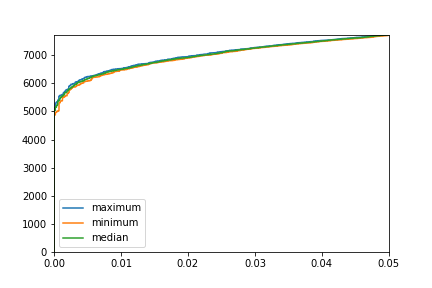
\includegraphics[width = \textwidth]{figures/MaxMinMedian_balancing.png}
		\caption{}
		\label{fig:results:maxminmedian_maintained}
	\end{subfigure}
	\caption[Results of maintaining the proportions of classes in the dataset]{}
	\label{fig:results:maxminmedian}
\end{figure}
\renewcommand{\baselinestretch}{1}

%used balancing: True, max AUCs: [343.2544021400075], min AUCs: [341.2731519815712], median AUCs: 342.3760451913073
%used balancing: False, max AUCs: [343.8859680229368], min AUCs: [342.05103793927975], median AUCs: 342.7538097947935
\subsubsection{Imputation}
\label{lab:results:imputation}
- Bei Imputation kam nichts heraus\\
\subsubsection{Splitting the Dataset}
\label{lab:results:splitting}
- Großer Unterschied wenn man den (großen) Datensatz nach XL/nXL oder sogar cross-linking target aufteilt\\

\subsection{Small datasets}
First, the smaller dataset was sampled using every $2^i$-th PSM, with $i$ being a natural number up to 13. This non-random approach ensures the appearance of PSMs originally classified as correct, but it also keeps the ratio of correct to incorrect PSMs. This leads to cases where only one or two PSMs appear, which originally were assigned a q-value of $<1\%$. \\
1. Experiment: Hints dass zu viele identifizierungen kommen wenn dataset zu klein und neue Metrik eingebaut\\
2. Experiment dann richtig\\
differing lengths of datasets dxl 7 p is because of filtration of ranks (?)
- Sinnvolle Plots zu Ratio Testing\\
- Neue Metrik erlaubt es der Implementierung, auch auf kleineren Datensätzen zu funktionieren